\section{Multiple Object Tracking}
\label{sec:MultipleObjectTracking}

This section continuously expands the previously started discussion on single object trackers. Our research originally targeted \gls{sot}, especially Siamese single object trackers. The plan to incorporate multiple objects remained only as a hypothesis to explore later since it brings a whole new set of challenges to overcome. However, thanks to our comprehensive survey on Siamese tracking~\cite{ondrasovic2021siamese}, we gained enough background knowledge to quickly absorb the newly emerging body of literature on a specific branch of multiple-object trackers that exploit Siamese architectures. We have to acknowledge that we did not compile a thorough \gls{sota} overview of \gls{mot} for the following reason. Our research is focused on Siamese neural networks, whereas the \gls{mot} is dominated by approaches that utilize detections + linking based on solutions exploiting a wide range of methods, from simple Munkre's algorithm~\cite{munkres1957assignment} through complicated graph formulations~\cite{chen2001motdynamicgraph} to even graph-based convolutional neural networks~\cite{papakis2021gcnnmatch}. Even though there are works that claim the use of Siamese neural networks in \gls{mot}, \egtext{}~\cite{cuan2018deepsiammot}, their utilization is in terms of \gls{reid} within the tracking-by-detection philosophy, for which Siamese networks are widely adopted. By Siamese tracking we explicitly mean the type of trackers described in \sectiontext{}~\ref{sec:SingleObjectTracking}. Nevertheless, we did not necesarily need as much background knowledge in \gls{mot} to identify that Siamese-based \gls{mot} is a freshly rising subfield of trackers we should contemplate exploiting due to its direct applicability to traffic analysis. As we will demonstrate, all the best practices from Siamese \gls{sot} have found their use in \gls{mot}, too.

% ##############################################################################
\subsection{Siamese-based Multiple Object Tracking}
\label{ssec:SiameseBasedMultipleObjectTracking}

Shuai~\etal{}~\cite{shuai2020multisiamrcnn} proposed a Siamese-based framework that can simultaneously handle object tracking, detection, and \gls{reid} (see \figtext{}~\ref{fig:MultiSiamRCNN}). The unification of all these aspects into a single pipeline is a significant advantage. In addition, the formulation allows the use of any Siamese tracker, which is a great contribution. Although this tracking system follows an inference pipeline similar to other tracking-by-detection systems, the distinction is that it does so based on cues generated by a single network. One important remark made by the authors is that that tracking by use of \gls{reid} alone is not robust enough to short-term changes, especially in the presence of partial occlusions. Our experiments will provide corroborating evidence, too.

% ------------------------------------------------------------------------------
\begin{figure}[!t]
    \centerline{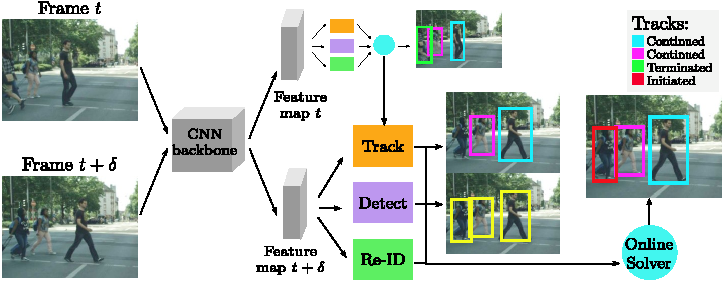
\includegraphics[width=\linewidth]{figures/theoretical_foundations/motsiam_trackrcnn_architecture.pdf}}
    \caption[Siamese \gls{mot} with track R-CNN]{Demonstration of how unification of the detection, tracking and \gls{reid} within a single architecture can be achieved. One important aspect that contributes to cost-effectiveness in terms of inference is that features required for all the mentioned tasks share the same backbone, which results in low
        computation and efficient runtime. \externalsrc{\cite{shuai2020multisiamrcnn}}}
    \label{fig:MultiSiamRCNN}
\end{figure}
% ------------------------------------------------------------------------------

From our point of view one trivial, but at the same time, very effective extension of the often-mentioned \siamfc{} tracker utilized $n$ exemplars to produce $n$ response maps and, therefore, to perform tracking of $n$ objects simultaneously~\cite{vaquero2021siammt}, aptly dubbed as \siammt{} (see \figtext{}~\ref{fig:SiamMTArchitecture}). The authors mentioned the incentive to develop their tracker to address the problem with running a costly detector for every frame to produce detections upon which another performance-demanding linking stage is usually executed. This framework was the first to demonstrate the qualities of a purely deep learning-based, end-to-end tracking pipeline capable of tracking multiple arbitrary objects at once. We believe this paradigm of tracking is yet to uncover its full potential.

% ------------------------------------------------------------------------------
\begin{figure}[!t]
    \centering
    \begin{subfigure}[b]{\textwidth}
        \centering
        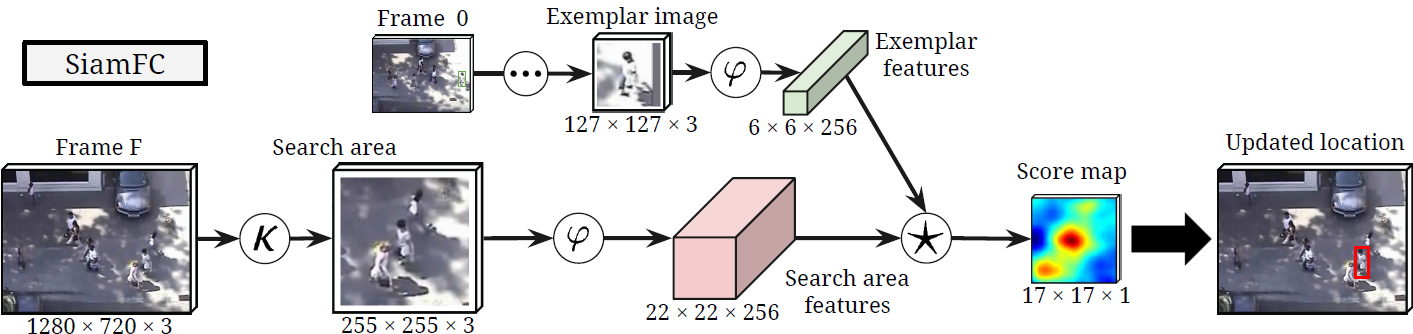
\includegraphics[width=\textwidth]{figures/theoretical_foundations/siammt_orig.png}
        \caption[]{}
    \end{subfigure}
    \begin{subfigure}[b]{\textwidth}
        \centering
        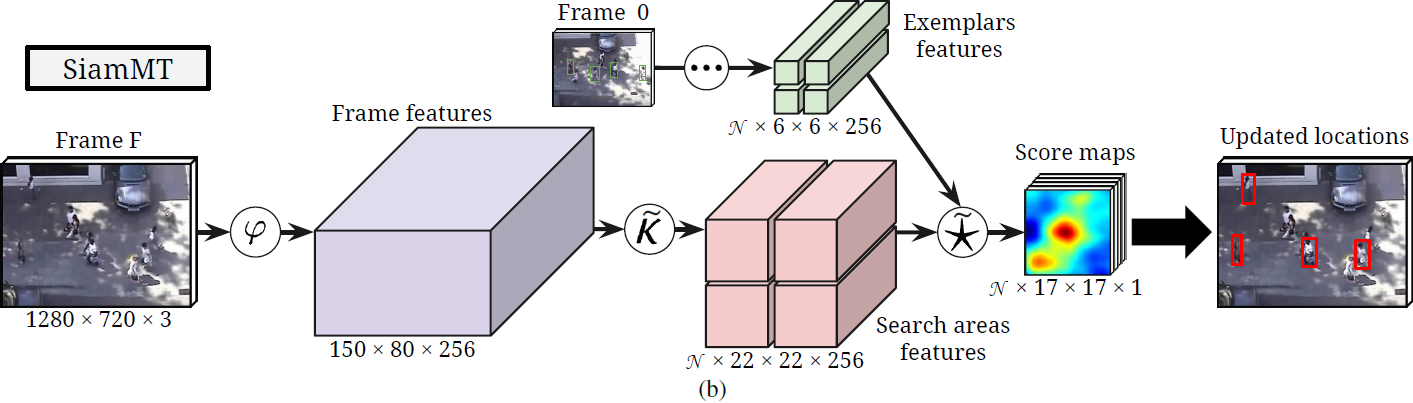
\includegraphics[width=\textwidth]{figures/theoretical_foundations/siammt_new.png}
        \caption[]{}
    \end{subfigure}
    \caption[\siammt{ architecture}]{The inference phase of the \imgpartdesc{a} \siamfc{} architecture to see the difference between the \imgpartdesc{b} \siammt{} successor. The \siammt{} framework first extracts features of the entire frame via the backbone $\varphi$. Subsequently, the obtained features belonging to distinct regions are cropped and resized using the $\tilde{K}$ operator, utilizing \gls{roi}-align operations. Finally, all these features are combined in the traditional cross-correlation way (although slightly adjusted to handle more objects) to produce a multiple-object response map indicating their predicted positions. \externalsrc{\cite{vaquero2021siammt}}}
    \label{fig:SiamMTArchitecture}
\end{figure}
% ------------------------------------------------------------------------------

The endeavor to exploit Siamese neural networks to assess the degree of similarity between two objects has spurred a plethora of proposals combining various mechanisms. Lee~\etal{}~\cite{lee2019motfpsn} combined Siamese similarity learning with \Glspl{fpn} (discussed in \sectiontext{}~\ref{ssec:FeaturePyramidNetworks}). This tracker still follows the path of tracking-by-detection paradigm, in which the similarity metric between the current detections and existing tracks plays an essential role. In this work, a criticism was raised concerning the plain Siamese architectures for not being sufficient for tracking owing to their structural simplicity and lack of motion information. To address the structural simplicity, a \gls{fpsn} was proposed. Then, in order to overcome the lack of motion information, additional spatiotemporal motion features were added to the \gls{fpsn} module.

% ------------------------------------------------------------------------------
\begin{figure}[!t]
    \centerline{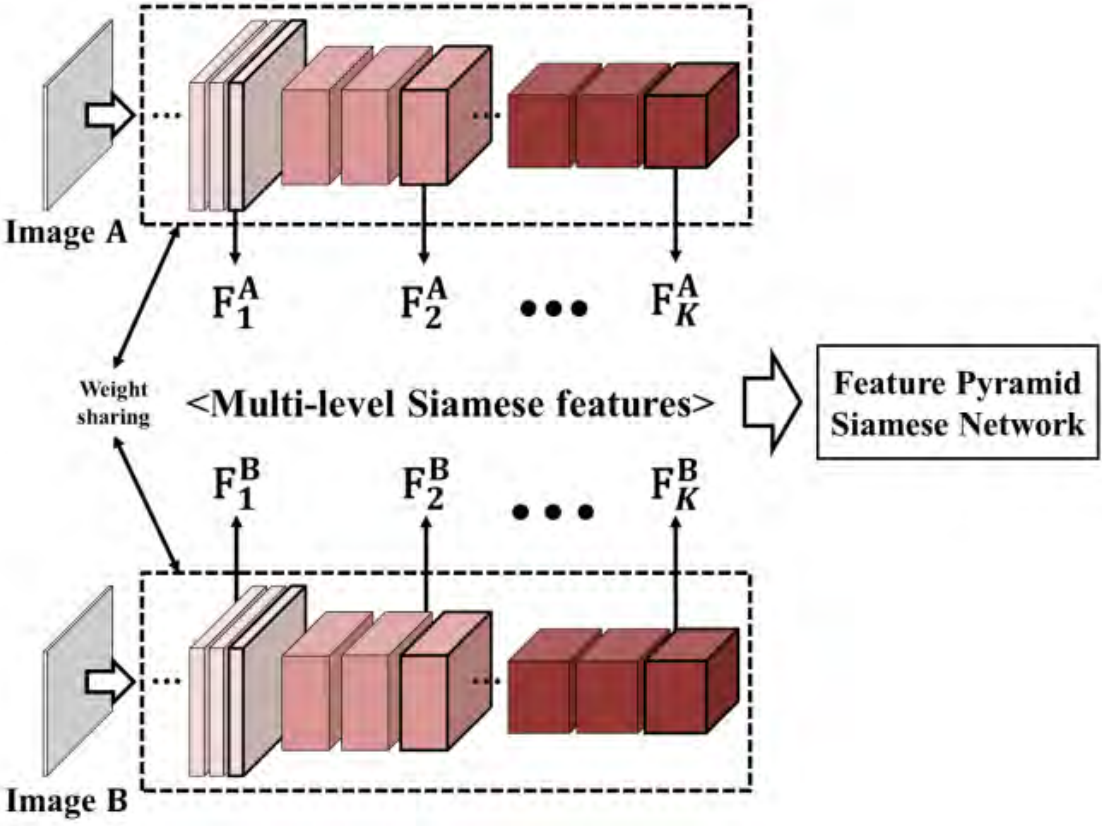
\includegraphics[width=0.7\linewidth]{figures/theoretical_foundations/feature_pyramid_siamese_network.png}}
    \caption[\Gls{fpsn} architecture]{A \gls{cnn} serving as a backbone that adopts Similarity learning as an enhancement to feature aggregation using \gls{fpn}. \externalsrc{\cite{lee2019motfpsn}}}
    \label{fig:FeaturePyramidSiameseNetwork}
\end{figure}
% ------------------------------------------------------------------------------

As a matter of fact, our research ended up with working with \siammot{}~\cite{shuai2021siammot} (Section~\ref{sec:SiamMOT}) architecture, which we will introduce in great detail later on. It is a multi-object tracker that practically encompasses some of the best approaches we have discussed so far into an end-to-end framework, such as Siamese tracker (multi-channel cross-correlation), \gls{rpn} head, centerness, feature fusion, and much more.